\chapter{Агенти}

Ово поглавље прелази са теоријских и инфраструктурних основа на конкретну архитектуру агената развијених у раду. Најпре се дефинише FinAsk агент: његова улога, општа архитектура и графички преглед. Након тога уводи се агент–судија као механизам евалуације квалитета одговора.

\section{FinAsk агент}

У овом одељку описан је дизајн LLM финансијског агента, уз образложење кључних одлука приликом његове изградње. Агент је осмишљен тако да аутономно спроводи анализу финансијских извештаја коришћењем више специјализованих алата. У наставку су наведене главне функционалности интегрисане у агента, као и разлози за њихово укључивање у систем.

\begin{figure}[!ht]
\centering
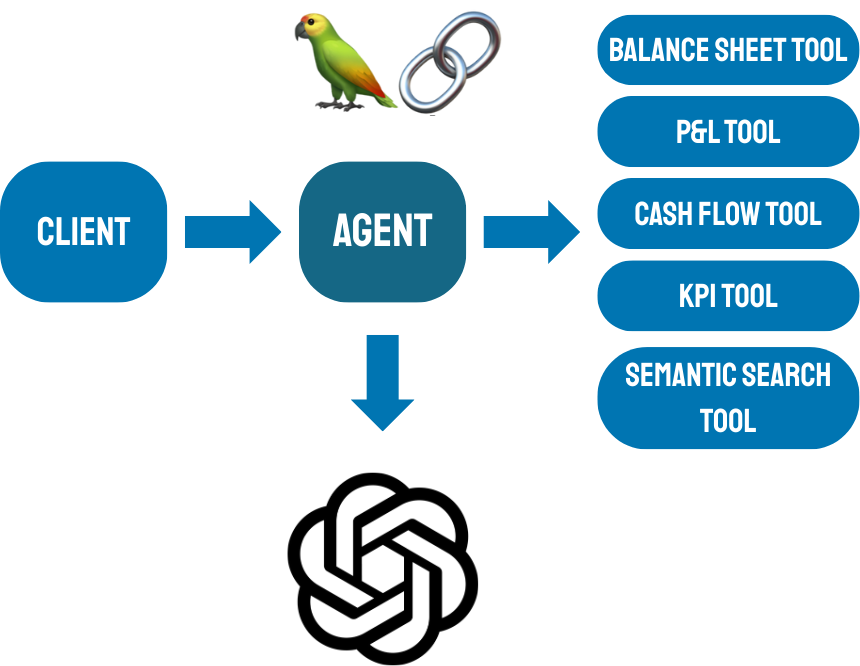
\includegraphics[width=0.8\textwidth]{images/agent.png}
\caption{Графички приказ архитектуре FinAsk агента}
\label{fig:agent_architecture}
\end{figure}

\subsection{Кључне функционалности агента}

Ради испуњавања захтева домена, идентификовано је шест кључних алата које наш агент користи:
\begin{enumerate}
    \item \textbf{Извлачење биланса стања:} Овај алат омогућава агенту да из финансијског извештаја издвоји структуриран биланс стања компаније. Парсирањем извештаја, агент проналази и извлачи главне категорије актива, пасива и капитала, враћајући их у облику погодном за даље рачунање. На тај начин, бројчани подаци о имовини, обавезама и капиталу постају директно доступни за анализу или одговарање на упите. Раздвајање биланса стања као посебног алата оправдано је тиме што гарантује прецизност у очитавању основних финансијских позиција и омогућава да се оне лако прослеђују другим компонентама система. За улаз прима период извештаја као и идентификатор паније, а излаз је приказан у наставку (Листинг \ref{lst:balance_sheet_json}).

    \begin{center}
    \begin{listing}[!ht]
    \begin{verbatim}
{
    "assets": {
        "current": 1200000,
        "non_current": 3000000,
        "total": 4200000
    },
    "liabilities": {
        "current": 1000000,
        "non_current": 2000000,
        "total": 3000000
    },
    "equity": {
        "total_equity": 1200000
    }
}
    \end{verbatim}
    \caption{Структурирани биланс стања (пример излаза алата)}\label{lst:balance_sheet_json}
    \end{listing}
    \end{center}

    \item \textbf{Извлачење биланса успеха:} Овај алат је задужен за прикупљање кључних података из биланса успеха. Агент путем њега дохвата приходе, расходе, нето добит, као и зараду по акцији (EPS) компаније. Ова функционалност је издвојена посебно јер обезбеђује да се показатељи пословног учинка прецизно извуку из извештаја. Структурирани приступ извлачењу прихода и расхода омогућава касније рачунање маржи, трендова и других метрика без ослањања на неструктурирани текст. За улаз прима период извештаја као и идентификатор паније, а излаз је приказан у наставку (Листинг \ref{lst:income_statement_json}).

    \begin{center}
    \begin{listing}[!ht]
    \begin{verbatim}
{
    "revenue": 5000000,
    "expenses": 4200000,
    "net_income": 800000,
    "EPS": 2.5
}
    \end{verbatim}
    \caption{Структурирани биланс успеха (пример излаза алата)}\label{lst:income_statement_json}
    \end{listing}
    \end{center}

    \item \textbf{Извештај о токовима готовине:} Трећи алат омогућава агенту да извуче податке из извештаја о токовима готовине. Конкретно, фокус је на три главне категорије новчаних токова: оперативни токови, инвестициони токови и финансијски токови. Агент издваја износ нето прилива/одлива готовине из пословања, улагања и финансирања, као и укупан нето промену готовине, што даје увид у то како компанија генерише и троши готовину. Укључивање овог алата је важно јер новчани токови пружају слику ликвидности и здравља пословања коју сами рачуни добити и губитка не откривају. Структурирани подаци о новчаним токовима омогућавају да се касније израчунају показатељи попут слободног новчаног тока или процени одрживост пословања. За улаз прима период извештаја као и идентификатор паније, а излаз је приказан у наставку (Листинг \ref{lst:cashflow_json}).

    \begin{center}
    \begin{listing}[!ht]
    \begin{verbatim}
{
    "cash_flow_from_operations": 900000,
    "cash_flow_from_investing": -200000,
    "cash_flow_from_financing": 100000,
    "net_change_in_cash": 800000
}
    \end{verbatim}
    \caption{Извод из извештаја о токовима готовине}\label{lst:cashflow_json}
    \end{listing}
    \end{center}

    \item \textbf{Извештај кључних показатеља:} Поред директног извлачења података, агент поседује алат за израчунавање кључних финансијских показатеља (енг. Key Performance Index - KPI) на основу прикупљених бројчаних вредности. Ова компонента рачуна индикаторе као што су повраћај на активу (енг. Return on Assets - ROA), повраћај на капитал (енг. Return on Equity - ROE), однос дуга и капитала (енг. debt-to-equity) и коефицијент текуће ликвидности (енг. current ratio). Алат преузима вредности из биланса стања и успеха које су добијене претходним алатима, и затим алгоритамски израчунава ове односе. Разлог за издвајање ове функционалности је да се обезбеди доследан и тачан прорачун финансијских индикатора, уместо да се ослонимо на LLM да их имплицитно рачуна из текста. Тако агент може кориснику директно да пружи увиде о профитабилности, ефикасности и ликвидности компаније. Ове показатељи су израчунати на основу позиција у билансима. За улаз прима идентификатор паније и период извештаја, а излаз је приказан у наставку (Листинг \ref{lst:kpi_json}).

    \begin{center}
    \begin{listing}[!ht]
    \begin{verbatim}
{
    "ROA": 0.19,
    "ROE": 0.67,
    "debt_to_equity": 2.5,
    "current_ratio": 1.2
}
    \end{verbatim}
    \caption{Пример израчунатих KPI показатеља}\label{lst:kpi_json}
    \end{listing}
    \end{center}

    \item \textbf{Семантичко претраживање (RAG алат):} Планирамо класичан RAG (енг. Retrieval-Augmented Generation) модул који омогућава агенту да претражује спољни извор знања на основу семантичке сличности упита. Овај алат служи као допуна постојећим функционалностима у случају да корисничко питање захтева информацију која није директно доступна кроз претходне алате, агент може да претражи релевантне документе и извуче одговарајући контекст. У основи, ова компонента користи векторску репрезентацију текста и семантичку претрагу да би идентификовала најрелевантније пасусе, чиме се проширује знање агента изван унапред дефинисаних поља.

    \begin{center}
    \begin{listing}[!ht]
    \begin{verbatim}
{
    "query": "Шта је проузроковало пораст прихода?",
    "result": {
        "text": "Менаџмент наводи да је пораст прихода резултат 
        веће потражње на тржишту и успешног лансирања новог 
        производа.",
        "source": "Годишњи извештај 2023 (MD&A одељак)"
    }
}
    \end{verbatim}
    \caption{RAG упит и пронађени контекст}\label{lst:rag_json}
    \end{listing}
    \end{center}
\end{enumerate}

Овако осмишљен скуп алата покрива и квантитативне и квалитативне аспекте анализе финансијског извештаја. Сваки алат је укључен са јасном сврхом: прва три обезбеђују да се кључни финансијски подаци прецизно и структурирано извуку, четврти пружа аутоматизовану аналитику кроз прорачун показатеља. Пети алат (семантичка претрага) додатно осигурава да агент може да дође до сваке информације која би могла бити упитана, а није директно обухваћена осталим алатима. Ова модуларна архитектура чини агента способним да одговори на разноврсна питања о финансијама компаније и оправдава сваку дизајнерску одлуку: специјализација алата повећава тачност, а њихова комбинација обезбеђује ширину покривених информација.

\subsection{Подршка за меморију}

Да бисмо омогућили будуће проширење функционалности, у плану је и додавање механизма меморије за агента. Подршка за меморију значи да ће агент бити у стању да памти релевантне информације током сесије или кроз више корака решавања задатка. На пример, агент би могао привремено чувати већ израчунате вредности или изведене закључке из ранијих корака анализе, како их не би прорачунавао више пута и како би разумео контекст сложенијих упита. Ова могућност је битна за сценарије у којима корисник поставља вишеструка повезана питања или када решавање једног задатка захтева низ међусобно повезаних корака. Додавањем меморије, агент постаје способан да води контекстуално свестан дијалог и да гради на претходно прикупљеним сазнањима, уместо да сваки пут креће од нуле.

Важно је, међутим, нагласити да у оквиру тренутне евалуације на скупу података меморија није пресудна компонента. Скуп задатака на којима тестирамо агента састоји се углавном од независних упита где сваки захтев може бити решен изоловано коришћењем наведених алата. То значи да агент, за потребе евалуације, не мора да памти резултате из једног упита да би решио следећи. Стога је подршка за меморију више унапређење ради будуће флексибилности него услов за тренутну функционалност. Ипак, предвиђањем оваквог механизма у дизајну, обезбеђујемо да је систем спреман за сложеније задатке и дијалошке сценарије који могу уследити након почетне фазе.

\subsection{Стратегија резоновања}

Приликом дизајнирања агента одлучено је за реактивни приступ резоновању. Ова одлука донета је након што је сагледана природа задатака у скупу података и сложеност упита. Већина захтева које агент треба да обради релативно су фокусирани (нпр. тражи се одређени финансијски показатељ или израчун на основу једног извештаја), те агенту обично није потребан дугачак низ корака да би дошао до одговора. Реактивни начин рада показао се довољним и ефикасним за овакве ситуације јер LLM може у једном кораку закључити који му је алат потребан (нпр. "извуци биланс стања", затим "обрачунај ROE") и добити одмах резултат, без формалног планирања целокупне стратегије. Поред једноставности, реактивни приступ је олакшао и развој и тестирање система, јер је лакше пратити и разумети ток одлучивања агента када он корак-по-корак образлаже и спроводи акције.

Насупрот томе, планско-извршни приступ би додао сложеност без јасне добити за домен. Морала би бити имплементирана додатна фаза планирања и морало би се веровати да ће LLM увек правилно исцртати план, што у нашим експериментима није довело до бољих резултата. Стога је закључено да је реактивни приступ примеренији: агент је у стању да брже и поузданије дође до решења финансијских упита ослањајући се на постепено резоновање и прилагођавање, што се показало успешним у евалуацији.



\section{Агент судија}

Оцењивање квалитета одговора на комплексна финансијска питања представља изазов, јер традиционалне метрике (попут процентуалне тачности или преклапања са референцом) често нису довољно осетљиве. За отворена питања постоји више валидних начина да се пружи исправан одговор, тако да једноставна поређења низова речи могу заказати \cite{evidently_ai_llm_judge_2025}. Са друге стране, ослањање на људске стручњаке за сваки одговор је споро и несразмерно скупо. Због тога се појавио приступ LLM-судија где се користи велики језички модел обучен да по унапред задатим критеријумима оцењује одговоре слично људском експерту \cite{zheng_judging_llm_2023,evidently_ai_llm_judge_2025}. У контексту финансијских анализа заснованих на 10-K извештајима компанија, LLM-судија делује као виртуелни финансијски судија, процењујући тачност и квалитет понуђених одговора у односу на проверене ``златне'' одговоре (енг. gold standard) стручњака.

\subsubsection{LLM као финансијски судија}

LLM-судија функционише тако што му се, уз оригинално питање, проследе и два одговора: одговор кандидата (који треба оценити) и референтни (златни) одговор. Модел затим, пратећи детаљна упутства, упоређује кандидатски одговор са референтним и процењује у којој мери се подударају, односно где кандидатски одговор одступа. Овај приступ се назива оцењивање у поређењу са златним стандардом и уобичајен је у задацима отвореног типа одговора где се тачан одговор зна унапред \cite{evidently_ai_llm_judge_2025}. У нашем случају, референтни одговор служи као поуздан оријентир на основу којег модел проверава чињенице, бројеве и логичку исправност у кандидатском одговору. На тај начин, LLM-судија може да ``разуме'' шта се очекује од идеалног одговора и да процени колико се дати одговор томе приближава. Овакав референтно вођен начин оцењивања показује се изводљивим и ефикасним, будући да су истраживања показала да модели-оцењивачи који имају увид у златни одговор могу донети оцене блиске људским судовима \cite{zheng_judging_llm_2023}.

Важно је истаћи да је LLM који се користи као судија у финансијском домену прилагођен да разуме специфичну терминологију и контекст. То значи да модел поседује довољно доменског знања о финансијама и 10-K извештајима, како би могао да ухвати нијансе у одговорима. Уколико се уз питање и одговоре додају и релевантни изводи из 10-K извештаја (контекстуалне информације), модел их такође користи приликом процене. Он проверава да ли се кандидатски одговор ослања на тај контекст и да ли је садржајно усаглашен са званичним подацима из извештаја, што додатно повећава тачност оцењивања.

\subsubsection{Критеријуми оцене одговора}

Оцењивање LLM-судије је структуирано према више унапред дефинисаних критеријума. У понуђеном упутству (prompt-у) експлицитно су наведени следећи аспекти, сваки са описом шта се очекује и скалом од 0 до 10:

\begin{enumerate}
    \item \textbf{Чињенична тачност (Factual Correctness)} -- Процена да ли су све изнете чињенице, финансијски подаци и бројке у кандидатском одговору тачни. Модел пореди конкретне цифре, процене и тврдње са референтним одговором и/или оригиналним подацима из 10-K. На пример, ако референтни одговор наводи приход од 5 милијарди долара, а кандидатски тврди 4 милијарде, LLM-судија ће то означити као фактичку грешку. Такође верификује прорачуне и да ли су извучени закључци у складу са чињеницама \cite{clearwater_analytics_2023}.

    \item \textbf{Потпуност (Completeness)} -- Оцењује да ли одговор обухвата све битне аспекте постављеног питања. Ако је питање сложено и има више подтема, добар одговор треба да се дотакне сваке од њих. LLM-судија упоређује обухват кандидатског одговора са дометом референтног: да ли је кандидат пропустио неки важан део или је дао површан одговор у односу на експертски \cite{evidently_ai_llm_judge_2025}. Виша оцена подразумева да је кандидатски одговор скоро једнако свеобухватан као и референтни, док се низак скор даје ако одговор изоставља значајне делове.

    \item \textbf{Финансијско расуђивање (Financial Reasoning)} -- Мери квалитет логике и аналитичког процеса у одговору. Модел анализира да ли кандидат правилно примењује финансијске принципе и методологије, да ли су објашњења уз бројке смислена и да ли закључци следе из изнетих података. Једноставно речено, оцена расуђивања одражава да ли одговор размишља као финансијски аналитичар. Упоређује се приступ из кандидатског одговора са референтним образложењем: нпр. ако референтни одговор образлаже кретање прихода анализирајући тржишне услове, а кандидатски одговор износи број без објашњења, то указује на слабије расуђивање. Добар финансијски судија модел идентификује такве разлике у дубини анализа.

    \item \textbf{Јасноћа (Clarity)} -- Оцењује квалитет презентације одговора: да ли је одговор добро организован, језички јасан и лак за разумевање. Финансијски подаци могу бити сложени, па је важно да одговор буде представљен прегледно, са логичним током мисли. LLM-судија анализира да ли кандидатски одговор следи структуру (нпр. увод, главни део, закључак), да ли користи примерен тон и стручну терминологију без непотребног жаргона, те да ли би циљна публика (нпр. инвеститори или пословни аналитичари) лако разумела излагање. Ово је једини критеријум који више гледа форму него садржину, али је важан за укупни утисак одговора.
\end{enumerate}

Сваки од ових критеријума модел оцењује по десетостепеној скали, где 0 означава најлошији могући учинак (потпуно нетачан или неразумљив одговор), а 10 репрезентује изванредан квалитет (потпуно исправан, комплетан и јасан одговор, раван експертском). Поред појединачних оцена, LLM-судија на крају изводи и укупну оцену, која представља заокружен суд о одговору у целини. Уједно даје и образложење за сваку оцену -- конкретна објашњења и примере који указују на јаке и слабе стране одговора. На пример, у образложењу за чињеничну тачност модел може навести: ``Кандидат је тачно навео приход компаније за 2022. (\$5,0 млрд према 10-K), али је погрешно приказао раст (тврди +15\% уместо +8\% годишње)''. Таква детаљност помаже да се идентификују кључне разлике у односу на референтни одговор и пружи корисна повратна информација кандидатима.

Важно је нагласити да су ови критеријуми и њихове дефиниције део системског упутства прослеђеног моделу. Истраживања су показала да пажљиво осмишљени рубрици (скупови критеријума са јасним описима) значајно побољшавају конзистентност и објективност оцењивања од стране LLM модела \cite{zheng_judging_llm_2023}. У нашем случају, модел добија прецизне смернице шта да тражи у одговору по сваком аспекту, што смањује произвољност у суду модела. Ово одражава праксу из најновијих оквира за аутоматско оцењивање, где се више атрибута (попут тачности, релевантности, кохерентности, образложења итд.) узима у обзир ради темељније оцене \cite{verga_replacing_judges_2024}. Такав мулти-димензионални приступ омогућава моделу да сагледа одговор из више углова, слично као што би то учинио људски судија-експерт.

\subsubsection{Процес оцењивања и логика модела}

Када се LLM-судији проследе питање, кандидатски и референтни одговор (уз опционе контекстуалне информације из 10-K извештаја), активира се унапред дефинисан процес резоновања модела. Мада је овај процес унутрашњи и невидљив директно, можемо га описати у корацима које би модел логички могао предузети:

\begin{enumerate}
    \item \textbf{Разумевање задатка и контекста:} Модел најпре прочита упутство које га поставља у улогу финансијског аналитичара-судије. Он ``зна'' да му је задатак да објективно упореди два одговора и оцени их према датим критеријумима. Затим пажљиво чита само питање како би разумео шта се тражи, као и додатне информације (нпр. изводе из 10-K) ако су обезбеђене. Ово осигурава да има пуни контекст пре него што погледа одговоре.

    \item \textbf{Читање и поређење одговора:} Модел чита референтни (експертски) одговор и кандидатски одговор. Током овога, он вероватно сегментира информације по тематским целинама или ставкама (нпр. одговор може имати делове о приходима, трошковима, стратегији раста итд.). Модел пореди одговоре део по део: за сваку кључну чињеницу или аргумент из референтног одговора проверава да ли је и како покривен у кандидатском. Такође бележи ако кандидат наводи нешто што стручни одговор није (то може бити додатна тачка или можда грешка). Ово двосмерно поређење омогућава детекцију и пропуста (ствари које недостају у кандидатском), и додатака (ствари које је кандидат можда измислио или погрешно извео).

    \item \textbf{Евалуација по критеријумима:} За сваки критеријум, модел примењује конкретна питања на прочитане одговоре:
    \begin{itemize}
        \item \textbf{Чињенична тачност:} ``Да ли се све бројке и тврдње у кандидатском одговору поклапају са информацијама из референтног одговора или датог контекста? Ако не, који су конкретни несагласни подаци?'' Модел упоређује вредности један-на-један (нпр. финансијски показатељи, процентуалне промене) и означава разлике.
        \item \textbf{Потпуност:} ``Да ли кандидат покрива све што и експерт? Постоје ли делови питања на које није одговорио?'' Модел идентификује сегменте из референтног одговора који немају еквивалент у кандидатском.
        \item \textbf{Финансијско расуђивање:} ``Да ли кандидат образлаже на сличан начин као експерт? Да ли је логика закључака исправна и поткрепљена подацима?'' Овде модел проверава конзистентност аргумената и да ли кандидат изводи исте или сличне закључке.
        \item \textbf{Нумеричка прецизност:} ``Да ли су све рачунске операције тачне?'' Модел може поновити једноставне прорачуне (ако су у одговору наведени) и проверити да ли кандидат није погрешно сумирао бројке или погрешно претворио валуте/јединице.
        \item \textbf{Јасноћа:} ``Да ли је одговор лако пратити и разумети? Постоји ли структура?'' Овде модел процењује стил писања: нпр. да ли кандидатски одговор почиње прегледом, да ли су мисли логично повезане, да ли су реченице јасне или превише сложене.
    \end{itemize}

    \item \textbf{Синтеза налаза и додела оцена:} На основу горе наведених анализа, LLM-судија сажима налазе за сваки критеријум. Он у текстуалном облику образлаже шта је пронашао: нпр. ``Под фактичком тачношћу: две вредности се не слажу са референтним одговором (грешка у нето приходу и стопи раста); Под потпуношћу: кандидат није поменуо анализу конкурентског окружења коју референтни одговор садржи; ...'' итд. После тога, модел преводи ове квалитативне налазе у нумеричке оцене 0-10 за сваки аспект. Оцењивање се врши у односу на референтни одговор као идеал: ако је кандидатски одговор готово идентичан по тачности и обухватности, добија високе оцене; ако значајно одступа, оцене су ниже. Коначно, модел одређује и укупну оцену, која није обичан просек већ целовита процена уз тежински осврт на све критеријуме.

    \item \textbf{Структурирани излаз:} Резултат који LLM-судија враћа форматиран је као JSON објекат са пољима за сваки критеријум и објашњењима, унапред дефинисан као захтев у упутству. Ова структура осигурава конзистенцију и лакшу машинску обраду.
\end{enumerate}

\begin{center}
\begin{listing}[!ht]
\begin{verbatim}
{
  "judge_evaluation": {
      "overall_score": 6,
      "criteria_scores": {
        "factual_correctness": 5,
        "completeness": 6,
        "financial_reasoning": 7,
        "clarity": 8
      },
      "criteria_explanations": {
        "factual_correctness": "The candidate lacks specific 
        figures from the 10-K filing, making accuracy 
        verification difficult.",
        "completeness": "The answer covers several aspects but 
        lacks numerical data for complete analysis.",
        "financial_reasoning": "Candidate shows solid understanding 
        of financial principles but lacks specific data.",
        "clarity": "Answer is well-structured and clearly 
        communicates the analysis process."
      },
      "overall_explanation": "The answer provides general analysis 
      but lacks specific numerical data and comparison with 
      reference answer.",
      "confidence": 0.7,
      "judge_model": "gpt-4o",
      "judge_tokens": null
    }
}
\end{verbatim}
\caption{Пример структурираног излаза LLM-судије}\label{lst:llm_judge_output}
\end{listing}
\end{center}

\subsubsection{Валидација приступа и релевантна истраживања}

Метод оцењивања одговора путем LLM-судије уз помоћ златних стандарда добио је велику пажњу у најновијим истраживањима. Резултати су охрабрујући: јаки LLM модели као што је GPT-4 показали су способност да се њихове оцене поклопе с људским експертским оценама у преко 80\% случајева -- што је отприлике на нивоу сагласности између два човека око истог одговора \cite{zheng_judging_llm_2023,evidently_ai_llm_judge_2025}. Другим речима, аутоматски судија се у великој већини случајева слаже са тим да ли је одговор добар или лош исто као што би се сложили и независни људски процењивачи. Ово сугерише да је LLM-судија скалабилна и поуздана метода за приближно хумано оцењивање отворених одговора \cite{evidently_ai_llm_judge_2025}, нарочито када је модел подешен да ублажи одређене предрасуде.

Истраживања су такође указала на неке изазове и предуслове за успешност оваквог система. На пример, модели могу испољити позициони предрасуду (наклоност првом одговору ако се пореде два), предрасуду према опширности (склоност да више цене дуже, развучене одговоре) или самоповлашћивање (тенденцију модела да преферира сопствене генерисане одговоре) \cite{zheng_judging_llm_2023,verga_replacing_judges_2024}. У нашем оквиру, где се вреднује један кандидатски одговор у односу на референтни, брижљиво састављен prompt помаже да се те пристрасности умање -- на пример, јасно се наводи да дужина одговора не сме утицати на оцену, како би се избегло неоправдано награђивање опширности. Такође, будући да је референтни одговор дат као оријентир, модел је вођен конкретним чињеницама, што смањује ризик од халуцинација или нагађања.

Детаљно дефинисање критеријума (попут нашег система са 5 категорија) показало се кључним за конзистентност: истраживање је уочило да у доменски специфичним задацима помаже дати моделу упутства шта чини добар одговор по сваком питању \cite{clearwater_analytics_2023}. Наш систем претпоставља да су референтни (златни) одговори већ доступни за свако питање -- што јесте додатни напор (припрема експертских одговора), али осигурава поуздано сидро за оцену. Алтернативно, за ситуације где нема комплетних златних одговора, могу се користити краће смернице (нпр. напомене за оцењивање) по питању \cite{verga_replacing_judges_2024}, како сугерише најновија пракса, мада то излази из оквира овог рада.

Коначно, више студија је потврдило да моделски оцењивачи могу боље ухватити нијансе квалитета одговора него једноставне метрике тачности. Verga и сар. у свом раду истичу да оцене од стране LLM-а имају јачу корелацију са људским судом од рецимо буквалног поклапања са златним одговором \cite{verga_replacing_judges_2024}. Све ово пружа уверење да је наша поставка -- LLM финансијски судија са рубриком и референтним одговором -- утемељена на провереним методама и способна да пружи објективне и детаљне евалуације. То је нарочито корисно у домену финансија где је тачност информација критична, а истовремено одговори могу бити отвореног типа где крути критеријуми не дају пуну слику.

Потпуни шаблон упутства (prompt-а) који се користи за LLM-судију дат је у Додатку \ref{appendix:llm_judge_prompt}.

